Este capítulo aborda a execução do método proposto por este trabalho e a análise dos resultados obtidos pelos experimentos realizados a fim de verificar a viabilidade do projeto, bem como sua eficiência.

\section{Planejamento dos experimentos}\label{sec:result_planejamento}
O intuito desta avaliação experimental é verificar a capacidade do sistema AutomailX de exibir um objeto 3D animado e classificar as ações do usuário a partir da leitura dos sensores do protótipo.

\todo{\textbf{Coesão:} ``Para este fim...''} Utilizou-se um Arduino Uno, um sensor MPU-6050 e um sensor flexível\todo{especificar sensores} para a captura dos dados de movimento do usuário. Todos estes equipamentos foram fixados \todo{qual o nome da luvinha de joelho} no joelho direito dos sujeitos de teste, simulando a pena que estaria utilizando a prótese.

Foram selecionados indivíduos para gerar o conjunto de dados que seria utilizado para a classificação, e solicitado para que cada um deles caminhasse em linha reta, enquanto era capturado o estado da transição de cada uma das ações. A captura foi feita a partir de um cabo USB conectado a um notebook \todo{configuração} estabelecendo conexão via porta serial para o programa.

As ações definidas para este experimento foram apenas voltadas à detecção de uma caminhada plana, classificando cada um dos passos de cada perna\todo{devido à limitação dos sensores disponíveis, pois o giroscópio não é tão preciso assim sozinho}{ }.

A simulação animada em 3D mostra em tempo real o movimento realizado pelos dois sensores e, após a captura dos dados, mostra também a ação realizada na prótese simulada, baseado na classificação dos dados de movimento.

\section{Execução dos experimentos}\label{sec:result_execucao}

\todo{Consertar imagem}\begin{figure}[ht]
	\caption{\label{fig:result_schem}Esquema das conexões}
	\begin{center}
	    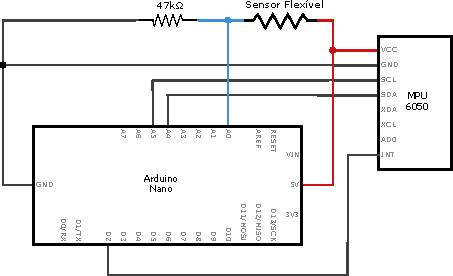
\includegraphics[width=.8\textwidth]{resources/result_schem}
	\end{center}
	\legend{Fonte: Elaborada pelo autor}
\end{figure}

\begin{figure}[ht]
	\caption{\label{fig:result_prototipo}Protótipo com o sensor flexível (a) e o MPU-6050 (b) conectados ao Arduino Nano}
	\begin{center}
	    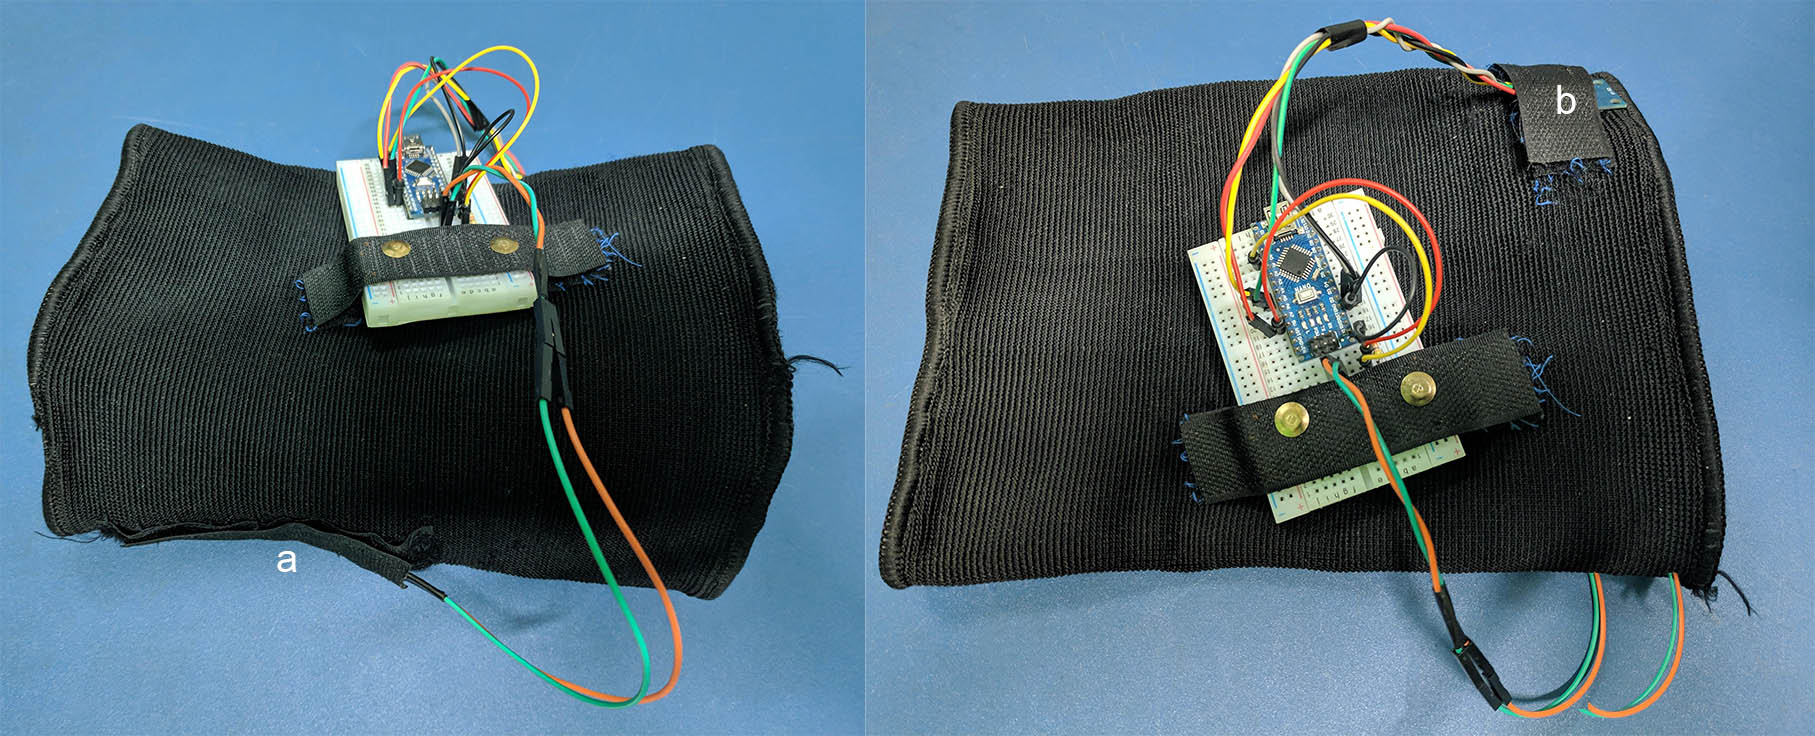
\includegraphics[width=.8\textwidth]{resources/result_prototipo}
	\end{center}
	\legend{Fonte: Elaborada pelo autor}
\end{figure}

\todo[inline]{Dado tal cenário, coletei os dados, funcionou mas poderia melhorar de tal jeito, isso e aquilo. Se não funcionou, pode ter sido limitação do classificador, ou do sensor, ou da placa.}
\todo[inline]{Escolha do algoritmo, comparação de gráficos
}